\section{Definisi GIS} 
Sistem Informasi Geografis atau disingkat SIG dalam bahasa Inggris Geographic Information System (disingkat GIS) merupakan sistem informasi khusus yang mengelola data yang memiliki informasi spasial (bereferensi keruangan). Atau dalam arti yang lebih sempit adalah sistem komputer yang memiliki kemampuan untuk membangun, menyimpan, mengelola dan menampilkan informasi bereferensi geografis atau data geospasial untuk mendukung pengambilan keputusan dalam perencanaan dan pengelolaan suatu wilayah, misalnya data yang diidentifikasi menurut lokasinya, dalam sebuah database. Para praktisi juga memasukkan orang yang membangun dan mengoperasikannya dan data sebagai bagian dari sistem ini. 
Teknologi Sistem Informasi Geografis dapat digunakan untuk investigasi ilmiah, pengelolaan sumber daya, perencanaan pembangunan, kartografi dan perencanaan rute. Misalnya, SIG bisa membantu perencana untuk secara cepat menghitung waktu tanggap darurat saat terjadi bencana alam, atau SIG dapat digunaan untuk mencari lahan basah (wetlands) yang membutuhkan perlindungan dari polusi atau dapat digunakan mencari informasi sebuah tempat khusus dan banyak manfaat lain yang dapat ikembangkan dalam sistem informasi geografis ini. 

\subsection{Pengertian GIS Menurut Para Ahli}
\begin{enumerate}

\item \textbf{Aronaff (1989)}
\subitem SIG adalah sistem informasi yang didasarkan pada kerja komputer yang memasukkan, mengelola, memanipulasi dan menganalisis data serta memberi uraian.

\item \textbf{Burrough (1986)}
\subitem SIG merupakan alat yang bermanfaat untuk pengumpulan, penimbunan, pengambilan kembali data yang diinginkan dan penayangan data keruangan yang berasal dari kenyataan dunia.

\item \textbf{Murai (1999)}
\subitem SIG sebagai sistem informasi yang digunakan untuk memasukkan, menyimpan, memanggil kembali, mengolah, menganalisis dan menghasilkan data bereferensi geografis atau data geospasial untuk mendukung pengambilan keputusan dalam perencanaan dan pengelolaan penggunaan lahan, sumber daya alam, lingkungan, transportasi, fasilitas kota, dan pelayanan umum lainnya.

\item \textbf{Marble et al (1983)}
\subitem SIG merupakan sistem penanganan data keruangan.  Bernhardsen (2002) SIG sebagai sistem komputer ang digunakan untuk memanipulasi data geografi. Sistem ini diimplementasikan dengan perangkat keras dan perangkat lunak komputer yang berfungsi untuk akusisi dan verifikasi data, kompilasi data, penyimpanan data, perubahan dan pembaharuan data, manajemen dan pertukaran data, manipulasi data, pemanggilan dan presentasi data serta analisa data.

\item \textbf{Gistut (1994)}
\subitem SIG adalah sistem yang dapat mendukung pengambilan keputusan spasial dan mampu mengintegrasikan deskripsi-deskripsi lokasi dengan karakteristik-karakteristik fenomena yang ditemukan di lokasi tersebut. SIG yang lengkap mencakup metodologi dan teknologi yang diperlukan, yaitu data spasial perangkat keras, perangkat lunak dan struktur organisasi  Berry (1988) SIG merupakan sistem informasi, referensi internal, serta otomatisasi data keruangan.

\item \textbf{Calkin dan Tomlison (1984)}
\subitem SIG merupakan sistem komputerisasi data yang penting.  Linden, (1987) SIG adalah sistem untuk pengelolaan, penyimpanan, pemrosesan (manipulasi), analisis dan penayangan data secara spasial terkait dengan muka bumi.

\item \textbf{Alter}
\subitem SIG adalah sistem informasi yang mendukung pengorganisasian data, sehingga dapat diakses dengan menunjuk daerah pada sebuah peta.

\item \textbf{Prahasta}
\subitem SIG merupakan sejenis software yang dapat digunakan untuk pemasukan, penyimpanan, manipulasi, menampilkan, dan keluaran informasi geografis berikut atribut-atributnya.  Petrus Paryono SIG adalah sistem berbasis komputer yang digunakan untuk menyimpan, manipulasi dan menganalisis informasi geografi. Dari definisi-definisi dari para ahli di atas dapat disimpulkan bahwa SIG merupakan pengelolaan data geografis yang didasarkan pada kerja komputer (mesin).

\item \textbf{Petrus Paryono}
\subitem SIG adalah sistem berbasis komputer yang digunakan untuk menyimpan, manipulasi dan menganalisis informasi geografi. Dari definisi-definisi dari para ahli di atas dapat disimpulkan bahwa SIG merupakan pengelolaan data geografis yang didasarkan pada kerja komputer (mesin).

\item \textbf{Chrisman (1997)}
\subitem SIG adalah sistem yang terdiri dari perangkat keras , perangkat lunak , data,manusia (brainware) organisasi dan lembaga yang digunakan untuk mengumpulkan,menyimpan,menganalisis dan menyebarkan informasi informasi mengenai daerah daerah di permukaan bumi.

\item \textbf{Lukman (1993)}
\subitem Menyatakan bahwa sistem informasi geografi menyajikan informasi keruangan beserta atributnya yang terdiri dari beberapa komponen utama yaitu:
\begin{enumerate}
\item Masukan data merupakan proses pemasukan data pada komputer dari peta (peta topografi dan peta tematik), data statistik, data hasil analisis penginderaan jauh data hasil pengolahan citra digital penginderaan jauh, dan lain-lain. Data-data spasial dan atribut baik dalam bentuk analog maupun data digital tersebut dikonversikan kedalam format yang diminta oleh perangkat lunak sehingga terbentuk basisdata (database).
\item Penyimpanan data dan pemanggilan kembali (data storage dan retrieval) ialah penyimpanan data pada komputer dan pemanggilan kembali dengan cepat (penampilan pada layar monitor dan dapat ditampilkan/cetak pada kertas).

\item Manipulasi data dan analisis ialah kegiatan yang dapat dilakukan berbagai macam perintah misalnya overlay antara dua tema peta, membuat buffer zone jarak tertentu dari suatu area atau titik dan sebagainya. Anon (2003) mengatakan bahwa manipulasi dan analisis data merupakan ciri utama dari SIG. Kemampuan SIG dalam melakukan analisis gabungan dari data spasial dan data atribut akan menghasilkan informasi yang berguna untuk berbagai aplikasi.

\item Pelaporan data ialah dapat menyajikan data dasar, data hasil pengolahan data dari model menjadi bentuk peta atau data tabular. Menurut Barus dan wiradisastra (2000) Bentuk produk suatu SIG dapat bervariasi baik dalam hal kualitas, keakuratan dan kemudahan pemakainya. Hasil ini dapat dibuat dalam bentuk peta-peta, tabel angka-angka: teks di atas kertas atau media lain (hard copy), atau dalam cetak lunak (seperti file elektronik).
\end{enumerate}

\item \textbf{Barus dan Wiradisastra (2000)} 
\subitem Mengungkapkan bahwa SIG adalah alat yang handal untuk menangani data spasial, dimana dalam SIG data dipelihara dalam bentuk digital sehingga data ini lebih padat dibanding dalam bentuk peta cetak, tabel atau dalam bentuk konvensional lainnya yang akhirnya akan mempercepat pekerjaan dan meringankan biaya yang diperlukan.
Sarana utama untuk penanganan data spasial adalah SIG. SIG didesain untuk menerima data spasial dalam jumlah besar dari berbagai sumber dan mengintergrasikannya menjadi sebuah informasi, salah satu jenis data ini adalah data pengindraan jauh. Pengindraan jauh mempunyai kemampuan menghasilkan data spasial yang susunan geometrinya mendekati keadaan sebenarnya dengan cepat dan dalam jumlah besar. 
SIG akan memberi nilai tambah pada kemampuan pengindraan jauh dalam menghasilkan data spasial yang besar dimana pemanfaatan data pengindraan jauh tersebut tergantung pada cara penanganan dan pengolahan data yang akan mengubahnya menjadi informasi yang berguna.

\item \textbf{Indrawati (2002)}
\subitem Aplikasi SIG dapat digunakan untuk berbagai kepentingan selama data yang diolah memiliki refrensi geografi, maksudnya data tersebut terdiri dari fenomena atau objek yang dapat disajikan dalam bentuk fisik serta memiliki lokasi keruangan.

\item \textbf{Dulbahri (1993)}
\subitem Tujuan pokok dari pemanfaatan Sistem Informasi Geografis adalah untuk mempermudah mendapatkan informasi yang telah diolah dan tersimpan sebagai atribut suatu lokasi atau obyek. Ciri utama data yang bisa dimanfaatkan dalam Sistem Informasi Geografis adalah data yang telah terikat dengan lokasi dan merupakan data dasar yang belum dispesifikasi.
\end{enumerate}

\section{Komponen Sistem Informasi Geografis}
Komponen-komponen pendukung SIG terdiri dari lima komponen yang bekerja secara terintegrasi yaitu perangkat keras (hardware), perangkat lunak (software), data, manusia, dan metode yang dapat diuraikan sebagai berikut:

\subsection{Perangkat Keras (Hardware)}
 Perangkat keras SIG adalah perangkat-perangkat fisik yang merupakan bagian dari sistem komputer yang mendukung analisis geografi dan pemetaan. Perangkat keras SIG mempunyai kemampuan untuk menyajikan citra dengan resolusi dan kecepatan yang tinggi serta mendukung operasi operasi basis data dengan volume data yang besar secara cepat. Perangkat keras SIG terdiri dari beberapa bagian untuk menginput data, mengolah data, dan mencetak hasil proses. Berikut ini pembagian berdasarkan proses :

\begin{enumerate}
\item CPU (unit pemroses utama). Perangkat ini merupakan bagian dari sistem komputer yang bertindak sebagai tempat untuk pemerosessan semua instruksi-instruksi dan program (processor). Selain itu, CPU juga berfungsi untuk mengendalikan seluruh operasi yang ada di dalam lingkungan sistem komputer yang bersangkutan. 

\item RAM. Perangkat ini digunakan oleh CPU untuk menyimpan (sementara) semua data dan program yang dimasukan melalui input device. Baik untuk jangka waktu yang panjang maupun pendek. Kebutuhan GIS mengenai RAM ini juga sangat bervariasi seperti halnya CPU di atas. 

\item Storage. Perangkat ini merupakan tempat penyimpanan data secara permanen atau semi permanen (temporary). Bila dibandingkan dengan RAM, akses pada media ini agak lambat. Harddisk,disket,CD-ROM,flash disk (yang terkoneksi melalui USB-port), dan pita magnetis merupakan contoh-contoh dari kelompok perangkat ini. Kebutuhan storage seperti ini sangat bervariasi mulai dari GIS yang satu ke GIS yang lain.

\item Input deivce. Perangkat ini merupakan peralatan-peralatan yang digunakan untuk memasukan data ke dalam perangkat GIS. Yang termasuk ke dalam perangkat ini adalah keyboard, mouse, digitaizer, scaner, kamera digital, dan sebagainya.

\item Output device. Perangkat ini merupakan peralatan-peralatan yang digunakan untuk merepresentasikan data dan atau informasi GIS. Yang termasuk ke dalam perangkat ini adalah layer monitor, printer plotter, dan sebagainya.

\item Peripheral (lainnya). Perangkat pelengkap ini merupaka bagian dari sistem komputer GIS yang belum termasuk ke dalam perangkat-perangkat yang telah di sebutkan di atas. Untuk GIS yang kecil dan sederhana peripheral kemungkinan sama sekali tidak diperlukan, tetapi untuk GIS yang besar apalagi menggunakan jaringan dan dapat di peresentasikan di jaringan internet (web), maka diperlukan kabel-kabel jaringan, modem, ISP, router, card jaringan/ ethernet, CPU khusus untuk clients dan server, dan sebagainya.
Pada saat ini GIS sudah dapat digunakan pada platform destkop, PC, laptop, workstation, dan multi-user host. Dengan demikian, fungsionalitas perangkat tidak terlalu terikat erat dengan karakteristik-karakteristik perangkat fisiknya. 

\end{enumerate}
\section{Komponen Sistem Informasi Geografis}
Komponen-komponen pendukung SIG terdiri dari lima komponen yang bekerja secara terintegrasi yaitu perangkat keras (hardware), perangkat lunak (software), data, manusia, dan metode yang dapat diuraikan sebagai berikut:

\subsection{Perangkat Keras (Hardware)}
 Perangkat keras SIG adalah perangkat-perangkat fisik yang merupakan bagian dari sistem komputer yang mendukung analisis geografi dan pemetaan. Perangkat keras SIG mempunyai kemampuan untuk menyajikan citra dengan resolusi dan kecepatan yang tinggi serta mendukung operasi operasi basis data dengan volume data yang besar secara cepat. Perangkat keras SIG terdiri dari beberapa bagian untuk menginput data, mengolah data, dan mencetak hasil proses. Berikut ini pembagian berdasarkan proses :

\begin{enumerate}
\item CPU (unit pemroses utama). Perangkat ini merupakan bagian dari sistem komputer yang bertindak sebagai tempat untuk pemerosessan semua instruksi-instruksi dan program (\textit{processor}). Selain itu, CPU juga berfungsi untuk mengendalikan seluruh operasi yang ada di dalam lingkungan sistem komputer yang bersangkutan.

\item RAM. Perangkat ini digunakan oleh CPU untuk menyimpan (sementara) semua data dan program yang dimasukan melalui \textit{input device}. Baik untuk jangka waktu yang panjang maupun pendek. Kebutuhan GIS mengenai RAM ini juga sangat bervariasi seperti halnya CPU di atas. 

\item Storage. Perangkat ini merupakan tempat penyimpanan data secara permanen atau semi permanen (\textit{temporary}). Bila dibandingkan dengan RAM, akses pada media ini agak lambat. Harddisk,disket,CD-ROM,flash disk (yang terkoneksi melalui USB-port), dan pita magnetis merupakan contoh-contoh dari kelompok perangkat ini. Kebutuhan storage seperti ini sangat bervariasi mulai dari GIS yang satu ke GIS yang lain.

\item Input deivce. Perangkat ini merupakan peralatan-peralatan yang digunakan untuk memasukan data ke dalam perangkat GIS. Yang termasuk ke dalam perangkat ini adalah \textit{keyboard, mouse, digitaizer, scaner,} kamera digital, dan sebagainya.

\item Output device. Perangkat ini merupakan peralatan-peralatan yang digunakan untuk merepresentasikan data dan atau informasi GIS. Yang termasuk ke dalam perangkat ini adalah layer monitor, printer plotter, dan sebagainya.

\item Peripheral (lainnya). Perangkat pelengkap ini merupaka bagian dari sistem komputer GIS yang belum termasuk ke dalam perangkat-perangkat yang telah di sebutkan di atas. Untuk GIS yang kecil dan sederhana peripheral kemungkinan sama sekali tidak diperlukan, tetapi untuk GIS yang besar apalagi menggunakan jaringan dan dapat di peresentasikan di jaringan internet (web), maka diperlukan kabel-kabel jaringan, modem, ISP, router, card jaringan/ ethernet, CPU khusus untuk \textit{clients} dan \textit{server}, dan sebagainya.
\end{enumerate}

\subsection{Perangkat Lunak (Software)}
Perangkat lunak digunakan untuk melakukan proses menyimpan, menganalisa, memvisualkan data-data baik data spasial maupun non-spasial. Pada sistem komputer modern, perangkat lunak yang digunakan biasanya tidak dapat berdiri sendiri, tetapi terdiri dari beberapa layer. Model layer ini terdiri dari perangkat lunak sistem operasi, program-program pendukung sistemsistem khusus (special system utilites), dan perangkat lunak aplikasi.Perangkat lunak yang harus terdapat dalam komponen software SIG adalah:
\begin{enumerate}
\item Alat untuk memasukkan dan memanipulasi data SIG
\item Data Base Management System (DBMS)
\end{enumerate}

Perangkat lunak khusus aplikasi GIS sering digunakan untuk menjalankan tugas-tugas GIS. Perangkat lunak tipe ini banyak tersedia dalam bentuk paketpaket perangkat lunak yang terkadang masing-masingnya terdiri dari multiprogram yang terintegrasi untuk mendukung kemampuan-kemampuan khusus untuk pemetaan dijital, manajemen, dan analisis data geografi. 

Pemilihan perangkat lunak GIS akan sangat bergantung pada sejumlah faktor, termasuk tujuan-tujuan penggunaan atau aplikasi, biaya pembelian dan pemeliharaan, kesiapan dan kemampuan personil-personil pengguna berserta agen perangkat lunak yang yang bersangkutan. 

\subsection{Data}
Pada prinsipnya terdapat dua jenis data untuk mendukung SIG yaitu :
\begin{enumerate}
\item Data Spasial
\subitem Data spasial adalah gambaran nyata suatu wilayah yang terdapat di permukaan bumi. Umumnya direpresentasikan berupa grafik, peta, gambar dengan format digital dan disimpan dalam bentuk koordinat x,y (vektor) atau dalam bentuk image (raster) yang memiliki nilai tertentu.
Sebagian besar data yang akan ditangani dalam SIG merupakan data spasial yang berorientasi geografis, memiliki sistem koordinat tertentu sebagai dasar referensinya dan mempunyai dua bagian penting yang membuatnya berbeda dari data lain, yaitu informasi lokasi (spasial) dan informasi deskriptif (attribute) yang dijelaskan berikut ini :

\begin{enumerate}
\item Informasi lokasi (spasial), berkaitan dengan suatu koordinat baik koordinat geografi (lintang dan bujur) dan koordinat XYZ, termasuk diantaranya informasi datum dan proyeksi.
\item Informasi deskriptif (atribut) atau informasi non spasial, suatu lokasi yang memiliki beberapa keterangan yang berkaitan dengannya, contohnya : jenis vegetasi, populasi, luasan, kode pos, dan sebagainya.
\end{enumerate}

Secara sederhana format dalam bahasa komputer berarti bentuk dan kode penyimpanan data yang berbeda antara file satu dengan lainnya. Dalam SIG, data spasial dapat direpresentasikan dalam dua format,yaitu:
\begin{enumerate}
\item Data Vektor
Data vektor merupakan bentuk bumi yang direpresentasikan ke dalam kumpulan garis, area (daerah yang dibatasi oleh garis yang berawal dan berakhir pada titik yang sama), titik dan nodes (merupakan titik perpotongan antara dua buah garis).Keuntungan utama dari format data vektor adalah ketepatan dalam merepresentasikan fitur titik, batasan dan garis lurus. Pada gambar \ref{data_vektor} merupakan tampilannya
\begin{figure}[ht]
\centering
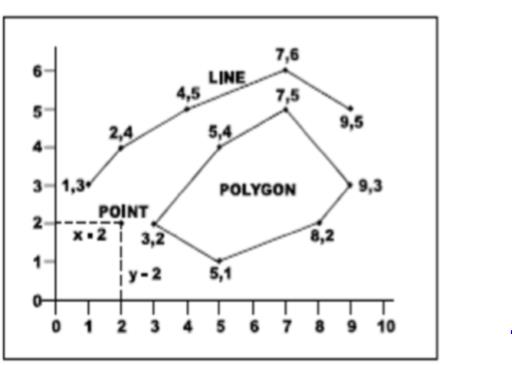
\includegraphics[width=0.5\textwidth]{pictures/data_vektor}
\caption{Data Vektor}
\label{data_vektor}
\end{figure}


\item Data Raster
Data raster (atau disebut juga dengan sel grid) adalah data yang dihasilkan dari sistem Penginderaan Jauh. Pada data raster,obyek geografis direpresentasikan sebagai struktur selgrid yang disebut dengan pixel(picture element). Pada gambar \ref{data_raster} merupakan tampilannya
\begin{figure}[ht]
\centering
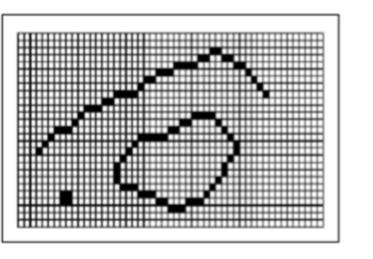
\includegraphics[width=0.5\textwidth]{pictures/data_raster}
\caption{Data Raster}
\label{data_raster}
\end{figure}
\end{enumerate}

\item Data Non Spasial (Atribut)
\subitem Data non spasial adalah data berbentuk tabel dimana tabel tersebut berisi informasi- informasi yang dimiliki oleh obyek dalam data spasial. Data tersebut berbentuk data tabular yang saling terintegrasi dengan data spasial yang ada.
Salah satu syarat SIG adalah data spasial, yang dapat diperoleh dari beberapa sumber antara lain:
\begin{enumerate}
\item Peta Analog
\subitem Peta analog (antara lain peta topografi, peta tanah dan sebagainya) yaitu peta dalam bentuk cetak. Pada umumnya peta analog dibuat dengan teknik kartografi, kemungkinan besar memiliki referensi spasial seperti koordinat, skala, arah mata angin dan sebagainya. Dalam tahapan SIG sebagai keperluan sumber data, peta analog dikonversi menjadi peta digital dengan cara format raster diubah menjadi format vektor melalui proses dijitasi sehingga dapat menunjukan koordinat sebenarnya dipermukaan bumi.

\item Data Sistem Penginderaan Jauh 
\subitem Penginderaan Jauh (antara lain citra satelit, foto udara dan sebagainya), merupakan sumber data yang terpenting bagi SIG karena ketersediaanya secara berkala dan mencakup area tertentu. Dengan adanya bermacam macam satelit di ruang angkasa dengan spesifikasinya masing masing, kita bisa memperoleh berbagai jenis citra satelit untuk beragam tujuan pemakaian. Data ini biasanya direpresentasikan dalam format raster.

\item Data Hasil Pengukuran Lapangan
\subitem  Data pengukuran lapangan yang dihasilkan berdasarkan teknik perhitungan tersendiri, pada umumnya data ini merupakan sumber data atribut contohnya: batas administrasi, batas kepemilikan lahan, batas persil, batas hak pengusahaan hutan dan lain - lain.

\item Data GPS (Global Positioning System)
\subitem Teknologi GPS memberikan terobosan penting dalam menyediakan data bagi SIG. Keakuratan pengukuran GPS semakin tinggi dengan berkembangnya teknologi. Data ini biasanya direpresentasikan dalam format vektor. 

\end{enumerate}
\end{enumerate}

\section{Ruang Lingkup Sistem Informasi Geografis}
Pada dasar nya sistem informasi geografis terdapat 6 proses yaitu:
\begin{enumerate}
\item Input data
\subitem Proses input data digunakan untuk menginputkan data spasial dan data non-spasial. Data spasial biasanya berupa peta analog. Untuk SIG harus menggunakan peta digital sehingga peta analog tersebut harus dikonversi ke dalam bentuk peta digital dengan menggunakan alat digitizer. Selain proses digitasi dapat juga dilakukan proses overlay dengan melakukan proses scanning pada peta analog.

\end{enumerate}

